\chapter{\label{sec:experimentation-and-evaluation}Experimentation and Evaluation}

% - trust explorer example
% - 9 fully functional modules
% - demonstrate the viability of run-time changes and alternative algorithmic approaches
% - open questions:
%   - how do we evaluate this?
%   - how do we show that it works as intended?
%   - we successfully bypassed the Android security model with protection against dynamic code injection using Webview
%   - pure technical (module loading times, memory usage impact, event-driven impact, event processing workload analysis, peak performance estimation)
%   - Github/NodeJS/Debian replacement workload analysis ("github is the largest code host in the world, with 20 million users and more than 57 million repositories"

This chapter will propose an experiment and evaluate the framework described in Section~\ref{sec:design}. The evaluation will be performed based on the result gathered from the experiment.

\section{Experiment}

The experiment consists out of conducting a use-case study, by creating a fully functioning example that demonstrates the composition and construction of an application with interchangeable trust models. This application will consist out of 6 components:

\begin{itemize}
	\item Test application GUI (view layer)
	\item Test application (logic layer)
	\item Trust algorithm 1 (logic layer)
	\item Trust algorithm 2 (logic layer)
	\item Execution engine (infrastructure layer)
	\item Transport engine (infrastructure layer)
\end{itemize}

Figure~\ref{fig:experiment} shows an overview of the example application. The domain of trust was chosen since this is a very interesting use-case that has not been explored yet in other works. It allows users of a system to define their own notion of the concept of trust and apply this to their system without requiring extensive knowledge about each application they are using. For this experiment, this work makes use of two different trust algorithms: Netflow and PimRank. These two algorithms act as an exampl for this experiment.

\begin{figure}[h]
	\centering
	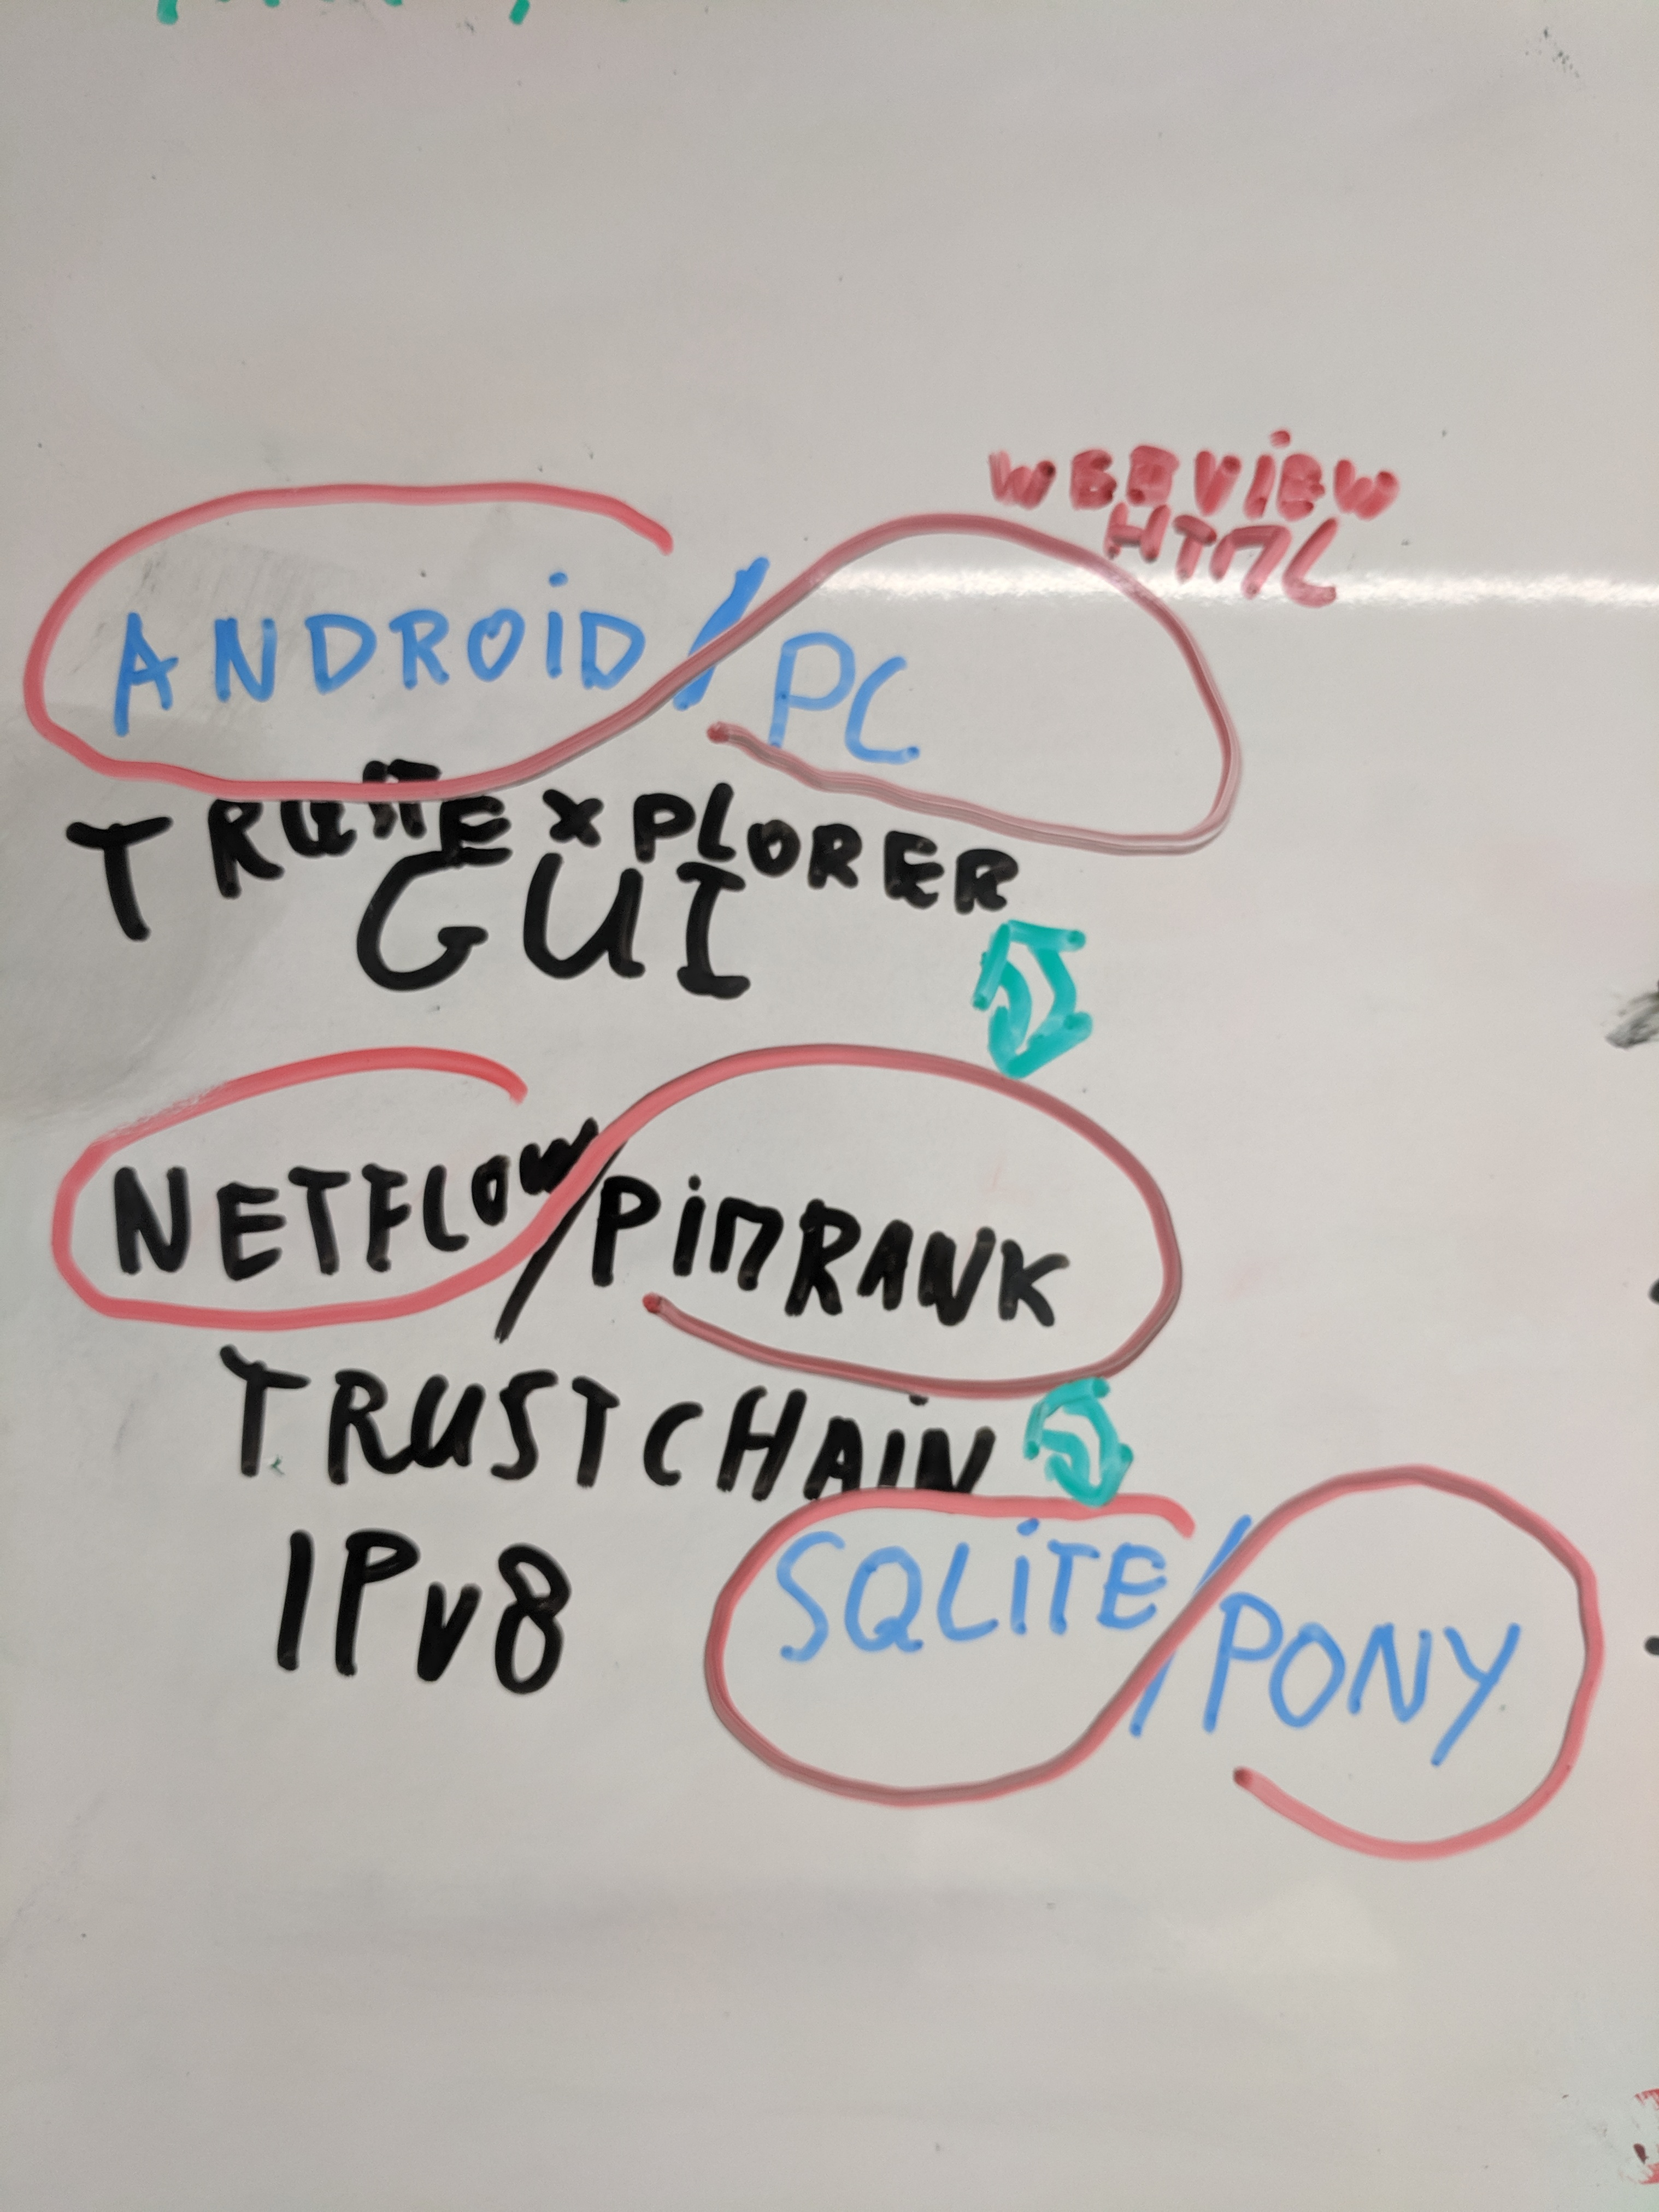
\includegraphics[width=0.5\textwidth]{images/experiment.jpg}
	\caption{\label{fig:experiment}}
\end{figure}